
%(BEGIN_QUESTION)
% Copyright 2009, Tony R. Kuphaldt, released under the Creative Commons Attribution License (v 1.0)
% This means you may do almost anything with this work of mine, so long as you give me proper credit

Explain how the following systems (analog electronic versus pneumatic) are similar in their behavior:

$$\includegraphics[width=15.5cm]{i03929x01.eps}$$

Calculate $V_{out}$ if $V_{in}$ = 3.4 volts.  Calculate $P_{out}$ if $P_{in}$ = 3.4 PSI.  Is the pneumatic system a {\it motion-balance} or a {\it force-balance} mechanism?

\vskip 10pt

Explain how the following systems (analog electronic versus pneumatic) are similar in their behavior:

$$\includegraphics[width=15.5cm]{i03929x02.eps}$$

Calculate $V_{out}$ if $V_{in}$ = 5.1 volts.  Calculate $P_{out}$ if $P_{in}$ = 5.1 PSI.  Is the pneumatic system a {\it motion-balance} or a {\it force-balance} mechanism?

\vskip 20pt \vbox{\hrule \hbox{\strut \vrule{} {\bf Suggestions for Socratic discussion} \vrule} \hrule}

\begin{itemize}
\item{} The distinction between force-balance and motion-balance is one that tends to confuse students.  A common tactical error students make is to attempt to memorize distinguishing characteristics in order to identify what type of balancing a particular mechanism employs.  A better approach is to {\it think through} the operation of such pneumatic mechanisms using ``thought experiments'' to identify which balance principle they employ.  Why do you think it is bad to go with the memorization approach instead of the ``thought experiment'' approach?
\item{} To many students, the 2:1 lever lengths in each example seem very confusing, because the lever lengths are opposite yet the gain in each case is identical.  For instance, in the top example the feedback has only {\it half} the lever length as the input, yet in the bottom example the feedback has {\it twice} the lever length as the input, yet these two different mechanisms exhibit the same overall gain.  How is this possible?
\item{} What difference does it make to us (as technicians) to know whether a mechanism is force- or motion-balance?  In other words, who cares???
\end{itemize}

\underbar{file i03929}
%(END_QUESTION)





%(BEGIN_ANSWER)

First example: $V_{out}$ = 6.8 volts ; $P_{out}$ = 6.8 PSI ; force-balance.

\vskip 10pt

Second example: $V_{out}$ = 10.2 volts ; $P_{out}$ = 10.2 PSI ; motion-balance.

%(END_ANSWER)





%(BEGIN_NOTES)


%INDEX% Reading assignment: Lessons In Industrial Instrumentation, Pneumatic Instrumentation (analogy to opamp circuits)

%(END_NOTES)


